\section{工业应用}
% 
% 
\subsection{生产环境神经网络部署}
\begin{frame}{工业应用——神经网络部署}
\begin{figure}[htp]
    \centering
    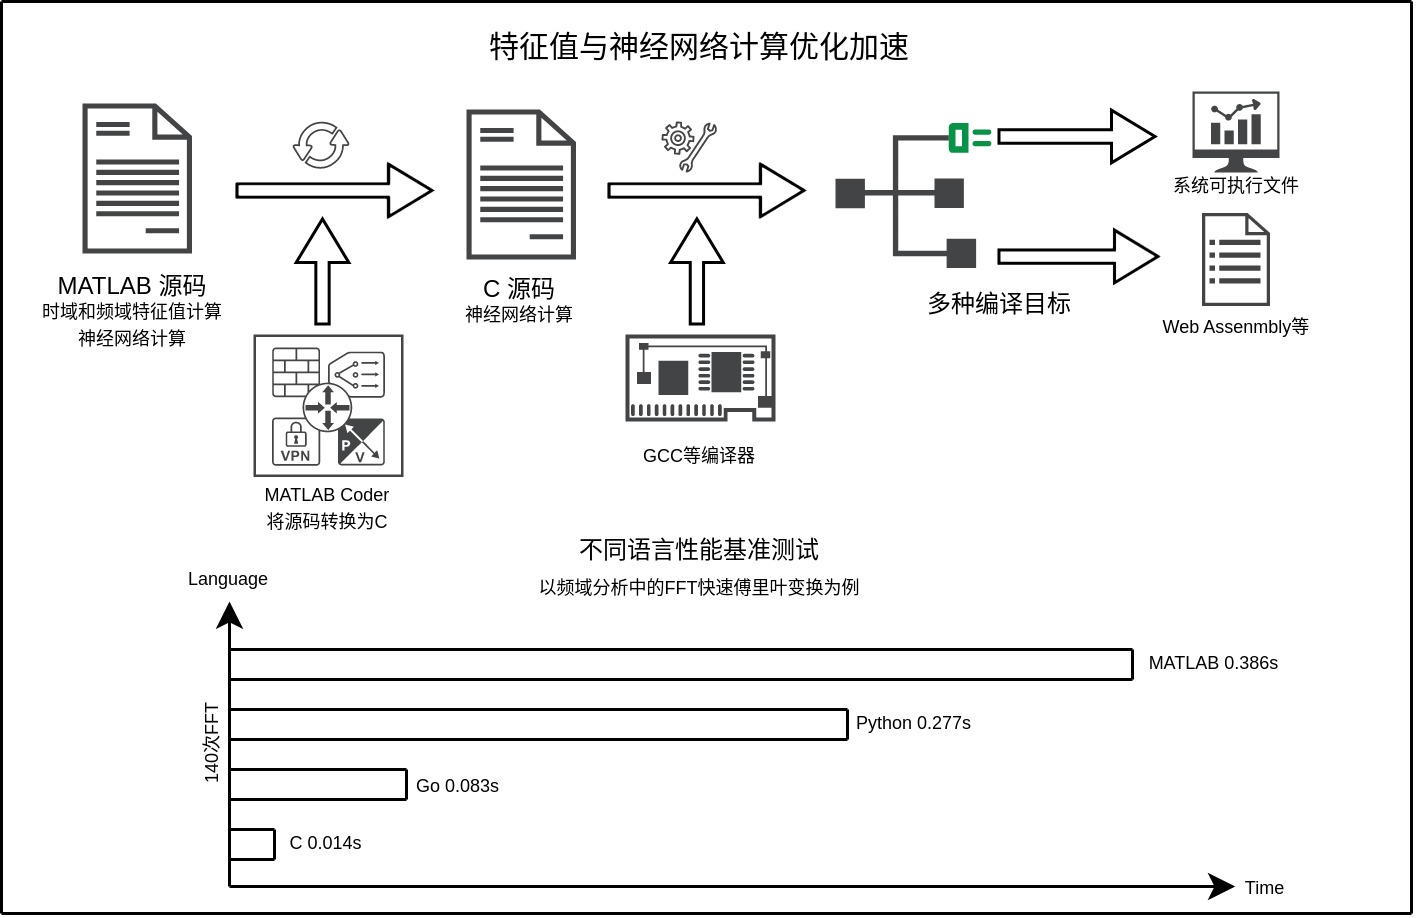
\includegraphics[width=11.5cm]{工业应用/compile_chain.jpg}
    % \caption{Matlab mill中的数据}
\end{figure}
\end{frame}
% 
% 
\subsection{车间工控网络\&备件库模型和制造执行系统}
\begin{frame}{工业应用——车间刀具磨损量工控网络}
% 
\begin{figure}[htp]
    \centering
    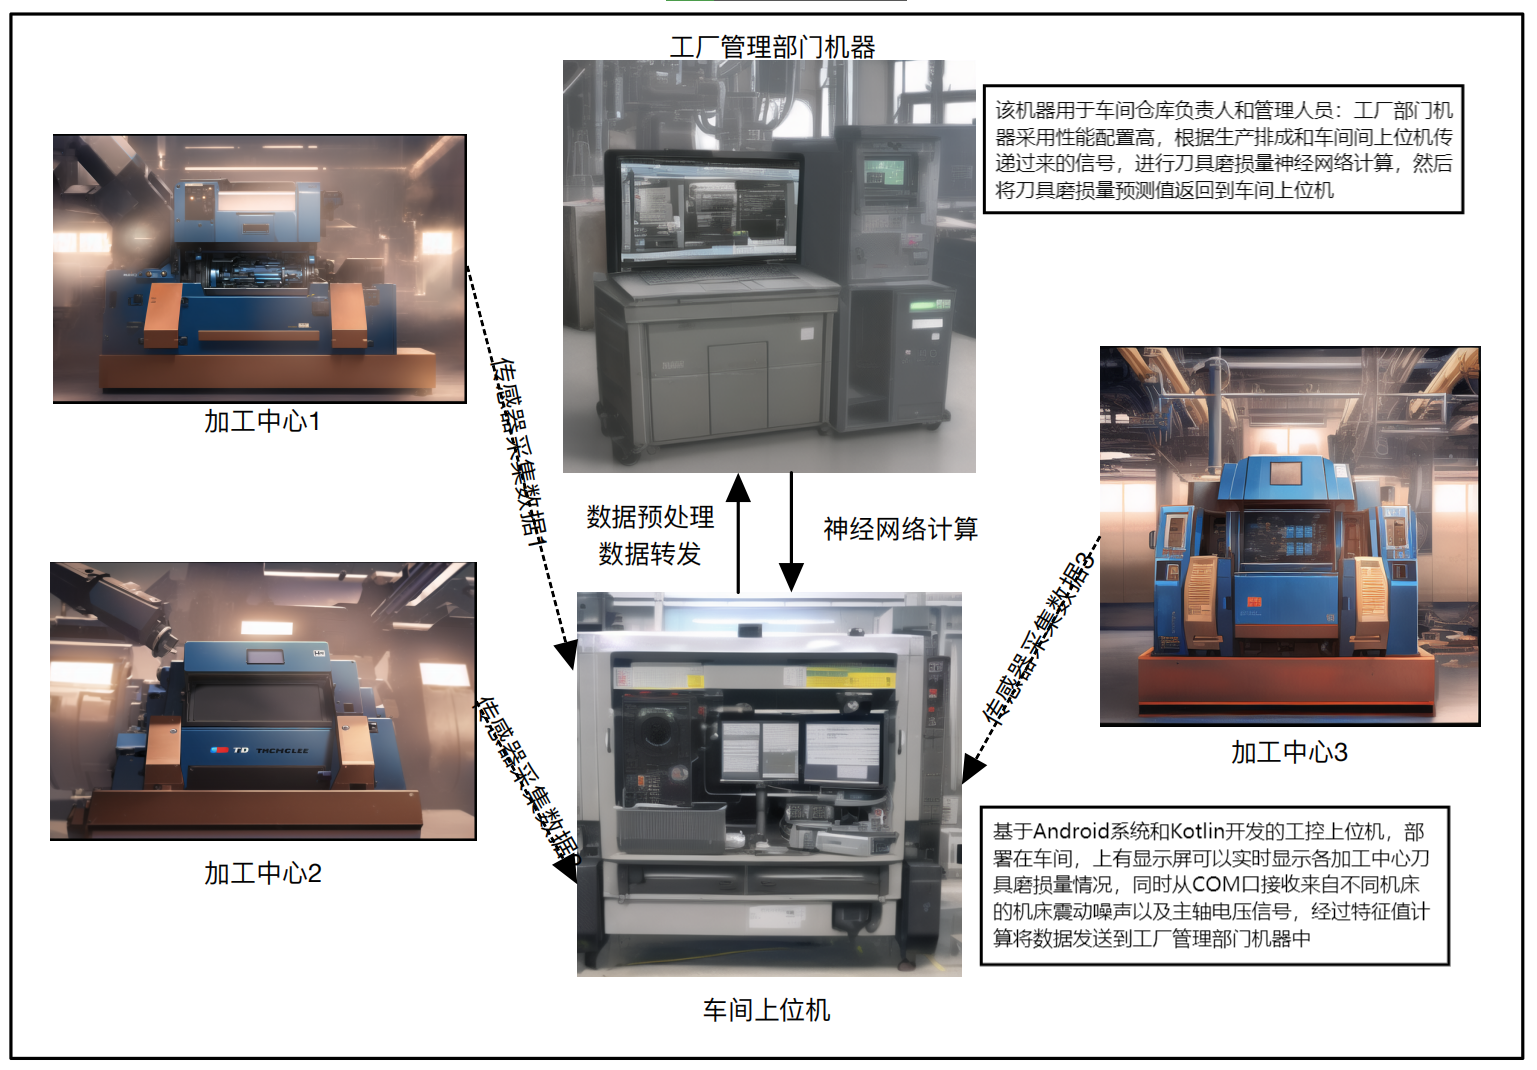
\includegraphics[width=11.5cm]{工业应用/车间网络.png}
    % \caption{Matlab mill中的数据}
\end{figure}
% 
\end{frame}

\begin{frame}{工业应用——备件库模型与制造执行系统}
% 
\ \ \ \ \ \ 通过对刀具磨损量的预测,可以做出在最优时机更换加工中心刀具的决策,减少停机检查时间和降低机加工次品率,提高加工产线的管理效率和生产水平,并最大化加工过程中的经济利益。
\begin{figure}[htp]
    \centering
    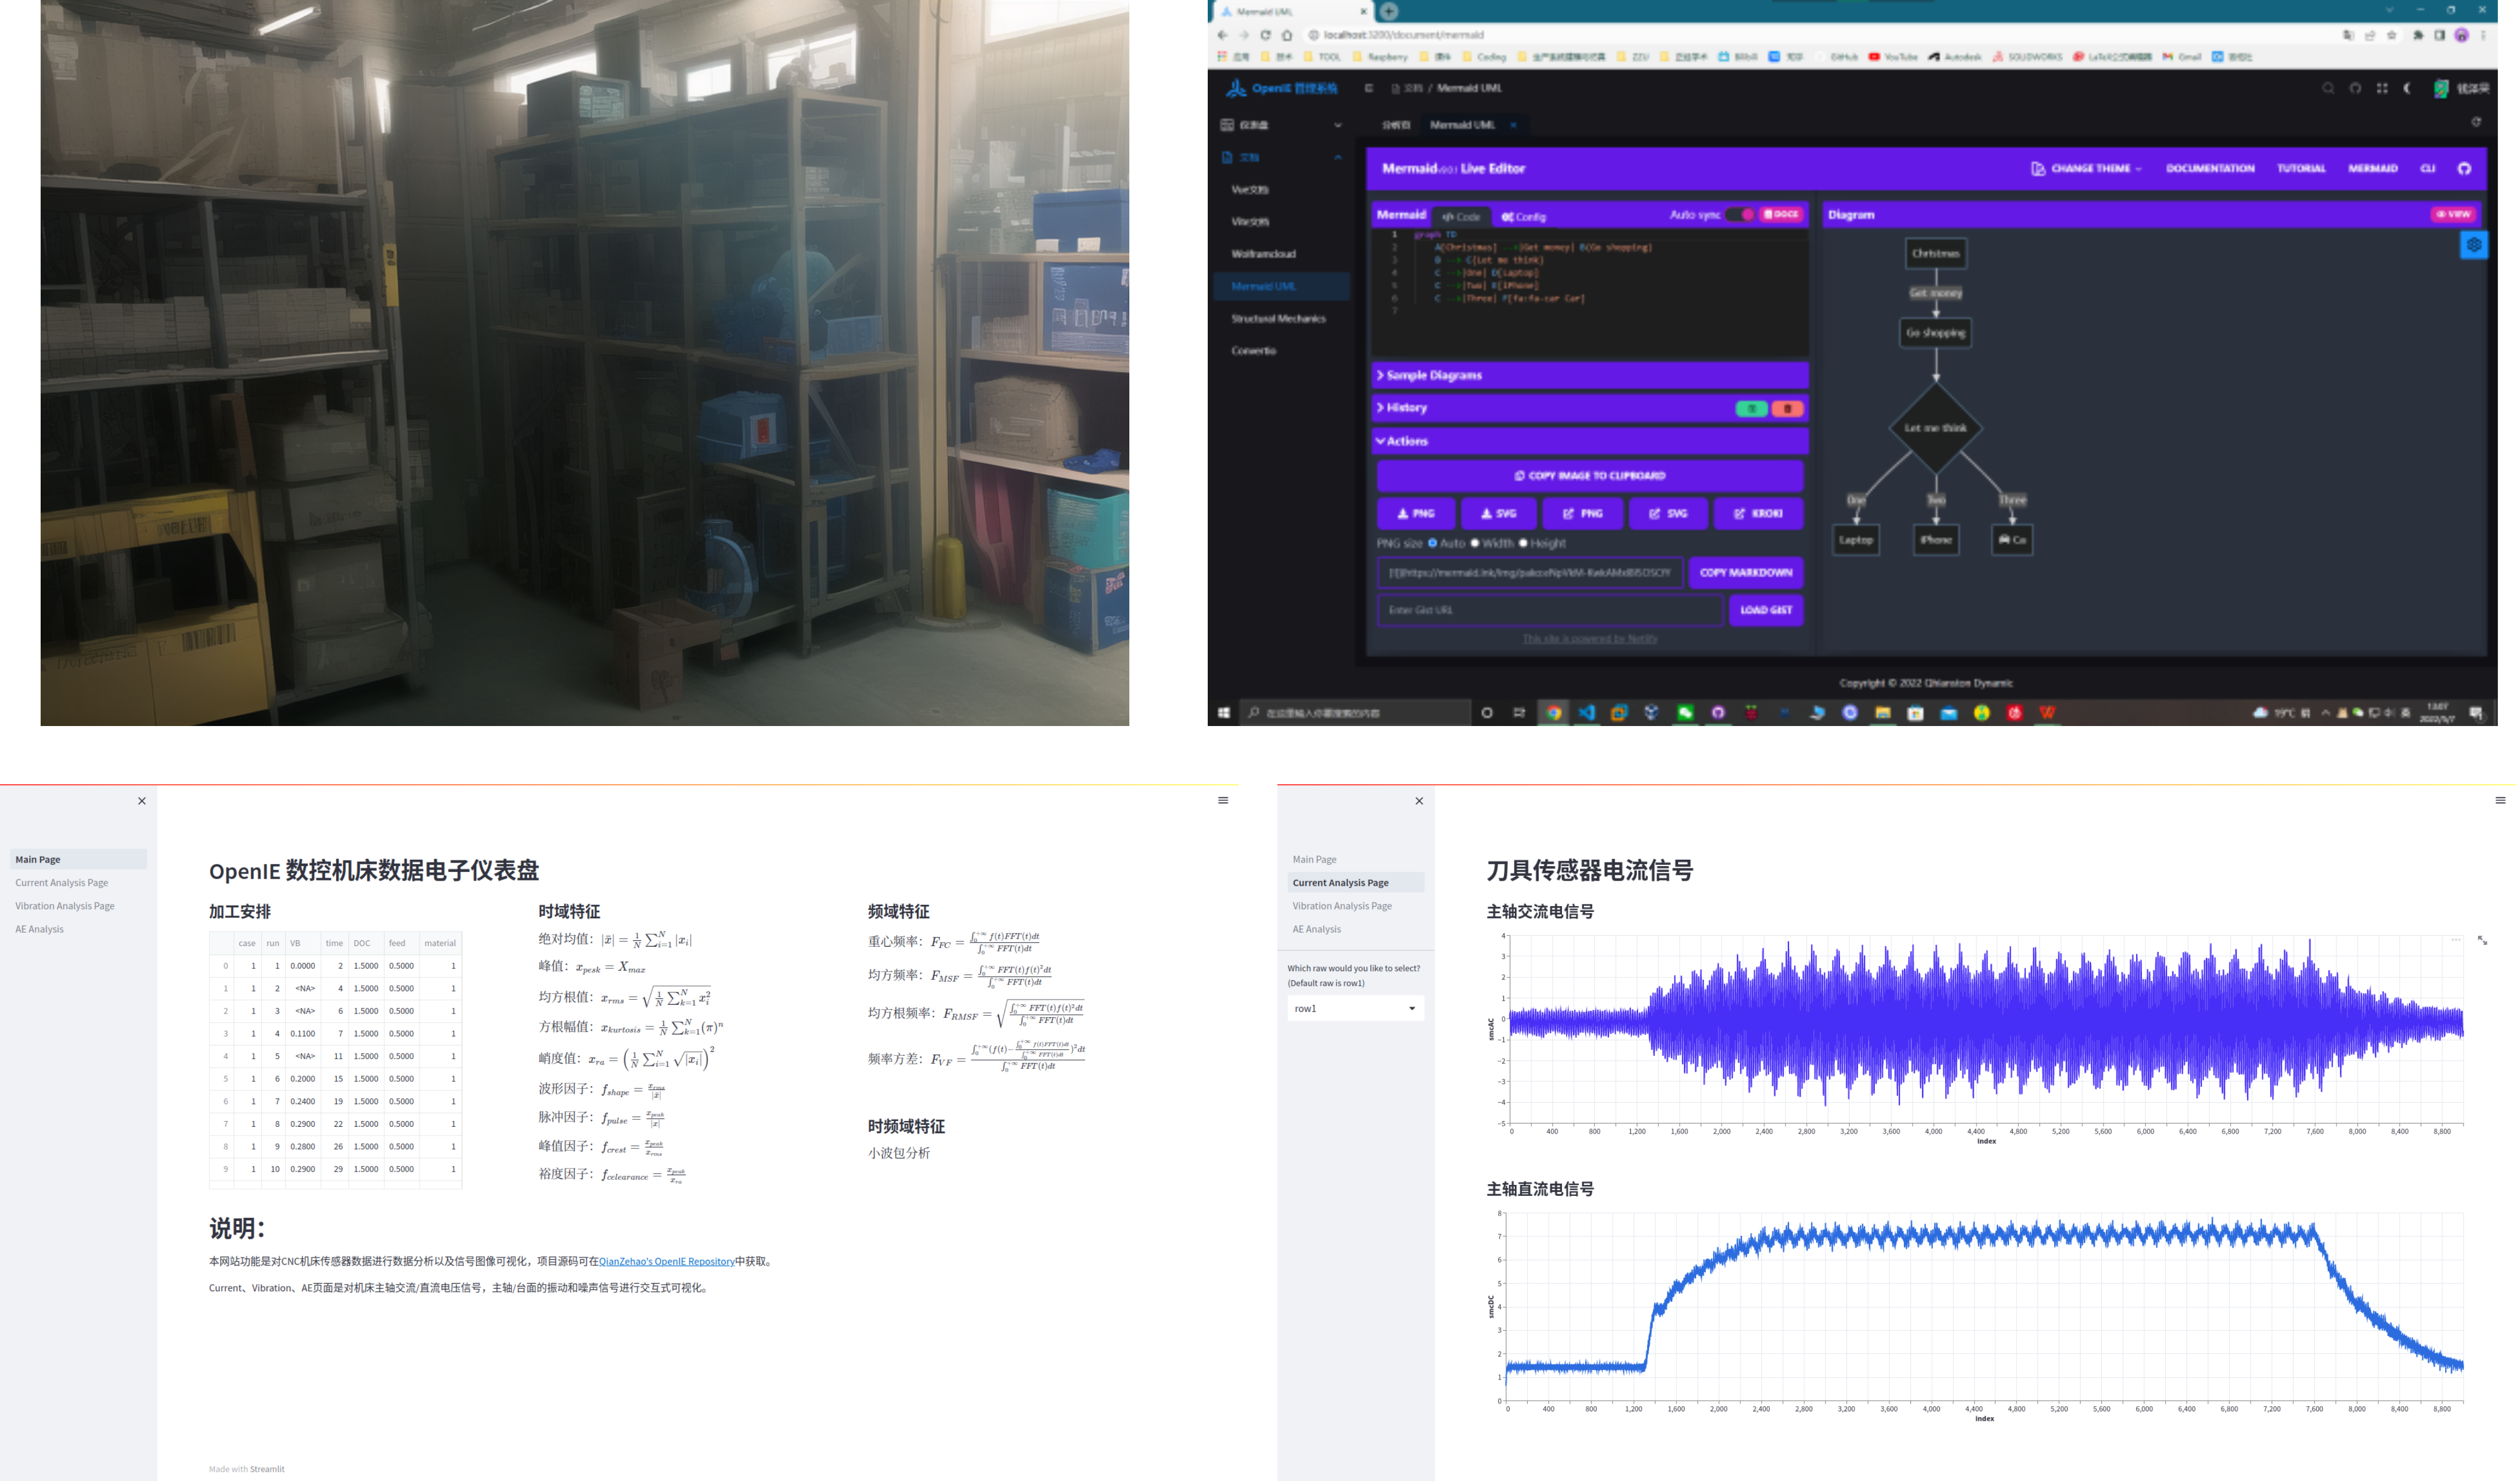
\includegraphics[width=10cm]{工业应用/openiecom.png}
    \caption{OpenIE刀具生命周期管理套件}
\end{figure}
% 
\end{frame}